%10/09 - Ruth Cobos
\chapter{Bases de datos}
\section{Introducción a las bases de datos relacionales}
En cualquier empresa o laboratorio, se va a necesitar acceder a una gran cantidad de datos. Los \textbf{sistemas de manejo de los datos (DBMS por sus siglas en inglés)} permiten tener todos los datos juntos y relacionados para facilitar su acceso, estando de forma conveniente y eficiente de usar. Las bases de datos pueden ser muy largas y tocan todos los aspectos de nuestras vidas, desde las transacciones bancarias al registro de notas de la universidad. 

El uso de bases de datos tiene muchas ventajas, como tener un acceso más sencillo a los datos que desde múltiples ficheros e integrar los datos. Utilizar ficheros aislados puede conllevar a datos redundantes e inconsistentes, aislamiento de los datos, atomicidad de las actualizaciones, concurrencia de los accesos y problemas de seguridad.

Existen bases de datos relacionales, en las cuales los modelos de datos son entidad-relación. Hay otros paradigmas como jerárquicas, no relacionales o basados en objetos.

Las arquitecturas suelen ser cliente-servidor, pero también puede ser paralela, distribuida o centralizada. En esta asignatura utilizaremos PostgreSQL, que es de arquitectura cliente-servidor.

A partir de la década de 1950 se empezó a hablar del almacenamiento de datos en cintas magnéticas. A finales de 1960, se empezó a guardar los datos, pero no fue hasta 1980 cuando se creó el lenguaje SQL. En 1990 empiezan a aparecer las redes, la web y el data mining. A principios de los 2000 comenzaron XML y XQuery. En el siglo actual hay millones de datos (big data).

\section{Modelo de entidad relacional}
\subsection{Esquema entidad-relación (ER)}
El esquema o diagrama entidad-relación (ER) es básicamente un gráfico que muestra de forma sencilla cómo se modela la problemática que se quiere abordar con una base de datos. Va a estar compuesto por un conjunto de entidades que pueden tener atributos que los describas. Entre las entidades hay relaciones. En un esquema ER, los rectángulos representan las entidades, los diamantes las relaciones, las elipses los atributos, las líneas unen los atributos con las entidades y las entidades entre sí, y el subrayado indica los atributos clave primarios. 

\begin{figure}[htbp]
\centering
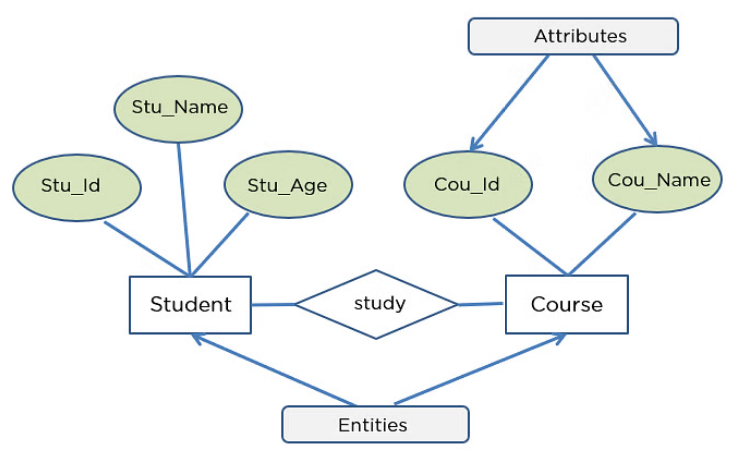
\includegraphics[width=0.5\linewidth]{figs/esquema-er.png}
\caption{Esquema ER.}
\end{figure}

Una \textbf{entidad} es un objeto o algo que pueda contener muchas instancias. Tiene atributos que le caracterizan y se deben poder distinguir de otras entidades mediante el contenido de los atributos. Normalmente, las entidades reciben un nombre en singular (por una sola palabra) y se representan con rectángulos. Las entidades débiles son aquellas cuya supervivencia depende de otra identidad.

Los \textbf{atributos} son propiedades de las entidades, y deben estar asignados a una entidad. El conjunto de valores para cada atributo se le conoce como dominio del atributo. Normalmente, los valores de los atributos son atómicos, es decir, indivisibles. 

Las \textbf{relaciones} son asociaciones entre las distintas entidades. Puede haber atributos en las relaciones. Las relaciones pueden ir también a la misma entidad en forma de bucle. En ese caso, se especifican los roles.

Es muy importante no poner en una entidad un atributo de otra entidad con la que esté relacionada.

\subsection{Claves primarias}
Una clave primaria permite identificar de manera única cada identidad. Puede ser uno o varios atributos. La clave candidata es la clave mínima primaria. Aunque puedan existir varias claves candidatas, solo una de ellas debería ser clave primaria. 

\subsection{Mapa de cardinalidades}
El mapa de cardinalidades expresa el número de entidades a los que se les puede asociar a otra entidad por una relación. Se representan por una flecha cuando es una relación individual o por una línea cuando son muchas. Hay tres cardinalidades: uno-a-uno (un cliente sólo puede pedir un préstamo, y un préstamo puede ser de un solo cliente), uno-a-muchos (un préstamo puede ser de un solo cliente, pero un cliente puede tener varios préstamos) o muchos-a-muchos (un cliente puede tener varios préstamos, y cada préstamo puede ser de varios clientes). 

\subsection{Especialización, jerarquía o generalización}
ISA se conoce como especialización, jerarquía o generalización. Viene del inglés "is a", y permite que una entidad se especialice en otras entidades. Aunque todas las entidades tengan los mismos atributos, después de la especialización las subentidades van a tener otros atributos y heredan los anteriores. Cuando en el esquema se va de arriba a abajo, se trata de una especialización, mientras que si se va de abajo a arriba se trata de una generalización. Sólo se heredan los atributos conforme se va especializando.

\subsection{Notación ER}

\begin{figure}[htbp]
\centering
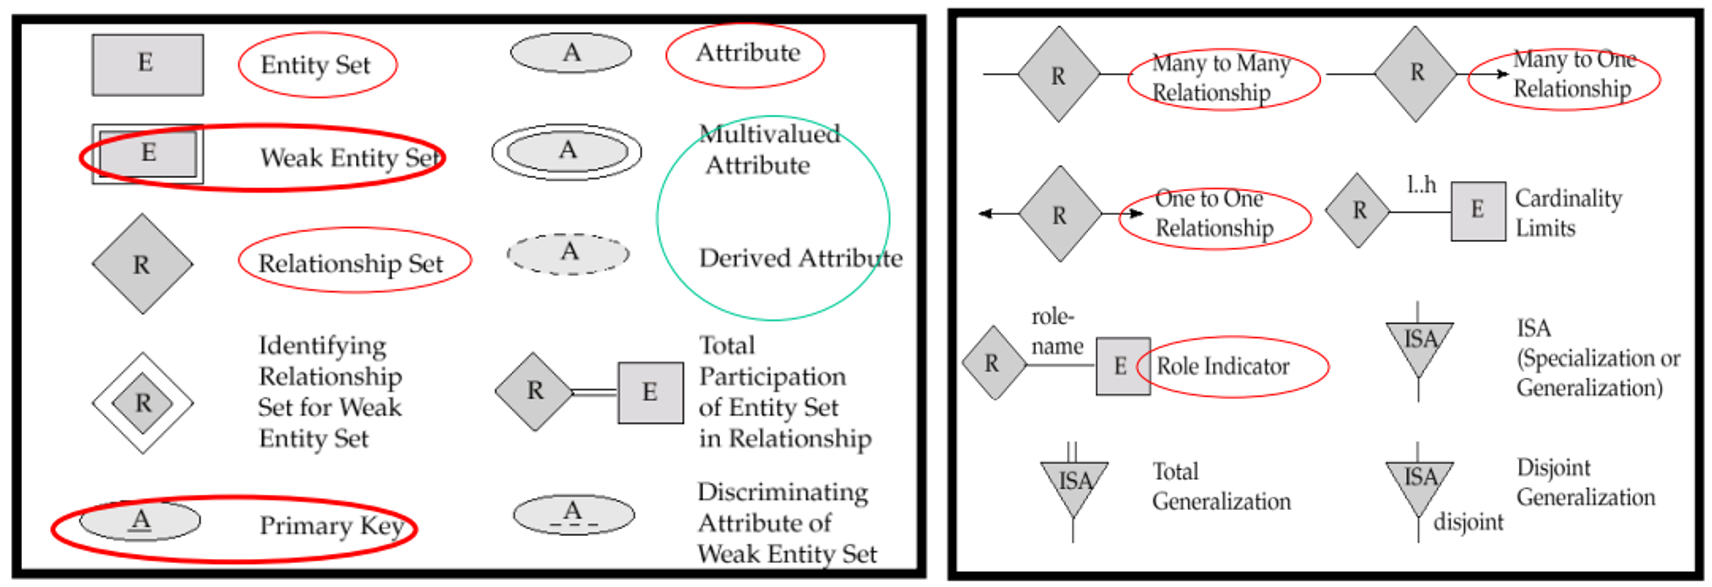
\includegraphics[width=\linewidth]{figs/notacion-er.png}
\caption{Resumen de la notación de un esquema ER. Los conceptos rodeados en rojo son los importantes. Los que están rodeados en azul no se recomiendan y los deberíamos evitar.}
\end{figure}

\subsection{Ejercicio 1: sistema de reserva de aulas para la universidad}
Vamos a hacer un sistema de reserva de salas para una universidad. Debe ser posible acceder al usuario que ha reservado cada sala, a las salas reservadas en un día concreto, o aulas concretas. Los profesores pueden reservar cualquier sala, pero los estudiantes solo pueden reservar las salas de propósito general o salas de seminario. Los usuarios se deben identificar por usuario y contraseña. 

\begin{figure}[htbp]
\centering
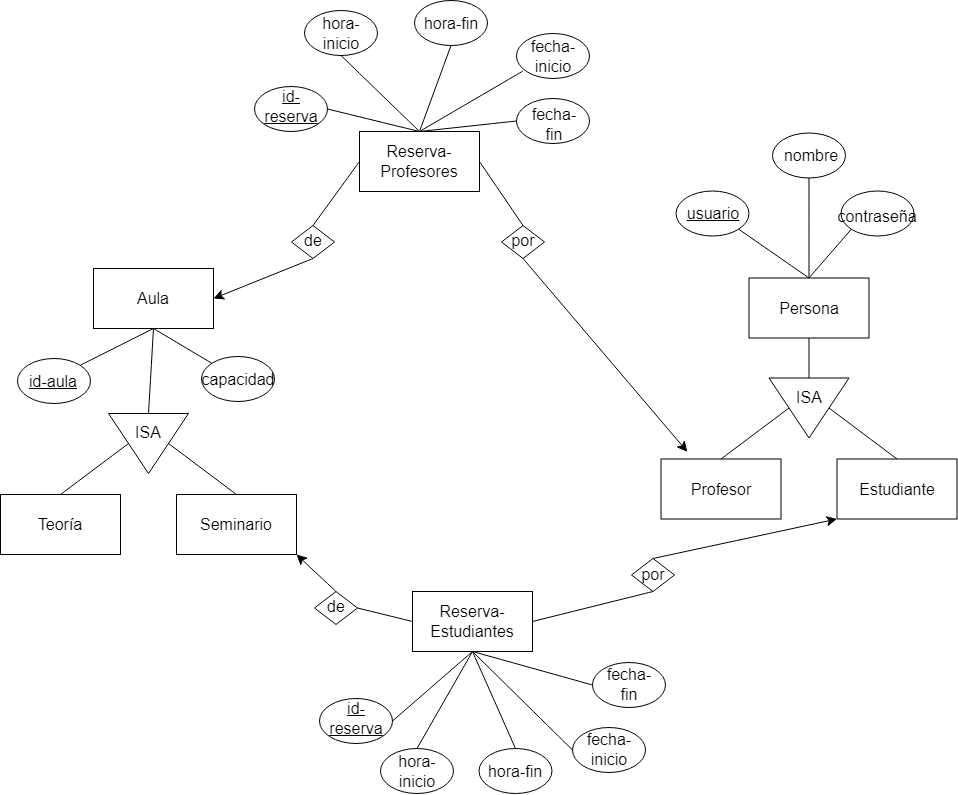
\includegraphics[width=0.7\linewidth]{figs/ejercicio-er-1.drawio.png}
\caption{Solución del ejercicio.}
\end{figure}

\subsection{Modelo relacional: esquema ER a tablas}
Desde el esquema ER, se debe convertir al modelo relacional o a un formato tabla. Para cada entidad hay una tabla única que tiene un número de columnas, que suele corresponder con los atributos, que tienen nombres únicos. Las relaciones n-n (muchos a muchos) tienen tablas separadas que consisten en las claves primarias de las dos identidades que relaciona. Las relaciones n-1 (muchos a uno) y 1-n (uno a muchos) pueden representar añadiendo un atributo extra en la parte de muchos que contenga la clave primaria de la parte uno.

A la hora de representar la especialización como tablas, hay dos opciones, y cada gestor lo hace de una manera: las especializaciones adquieren solo la clave primaria o adquiere todos los atributos de la generalización.

Los pasos para crear tablas son:
\begin{enumerate}
\item Identificar las claves primarias
\item Identificar entidades
\item Identificar los atributos redundantes de las entidades y especializar
\item Identificar relaciones n-n
\item Todas las entidades producen una tabla
\item Todas las relaciones n-n producen una tabla
\item Todas las relaciones n-1 añaden una columna a la entidad n.
\end{enumerate}

\subsection{Resumen}
El primer paso es crear el esquema ER identificando las entidades con sus atributos y relaciones, las cardinalidades y las especializaciones. Después, se debe reducir el esquema a tablas, identificando las claves primarias, entidades y relaciones n-n. Las entidades y las relaciones n-n producen una tabla. Todas las relaciones n-1 añaden columnas a la entidad de muchos.

\subsection{Ejercicio 2: gestión de mercancías}
Una empresa de gestión de mercancías desea tener almacenados los datos de sus clientes, los productos y los proveedores relacionados con los distintos pedidos que realizan los clientes. También interesa llevar un control sobre los tipos de los productos.

\begin{figure}[htbp]
\centering
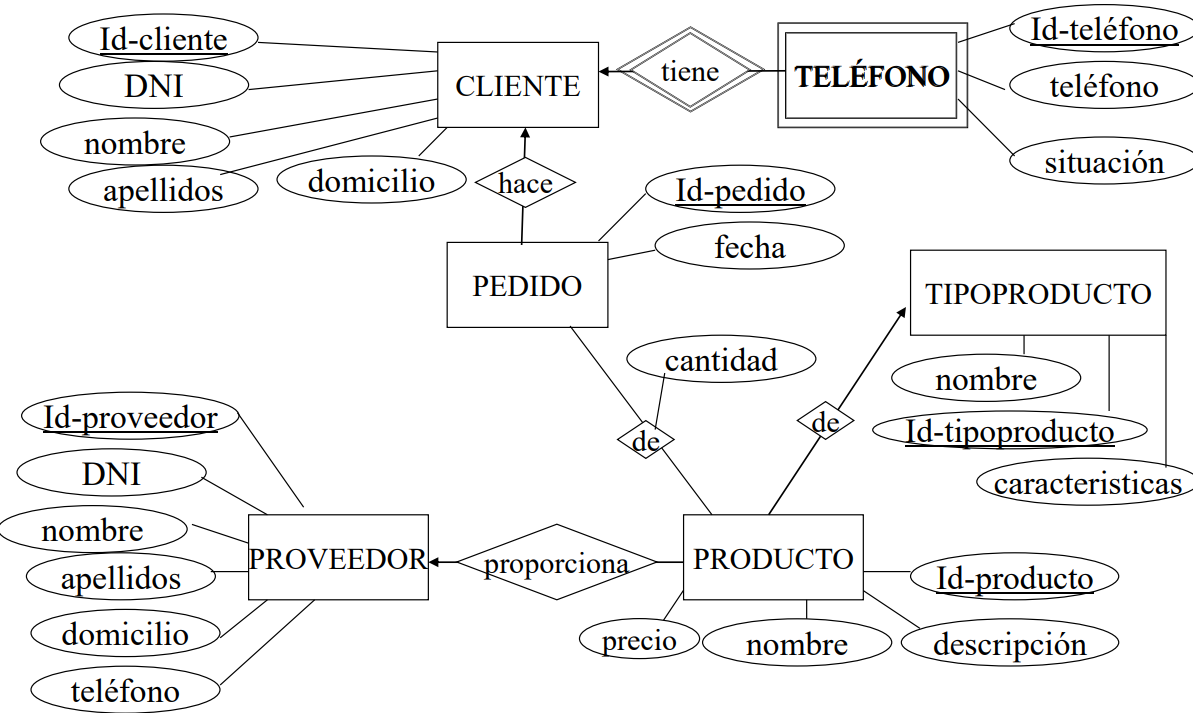
\includegraphics[width=0.7\linewidth]{figs/ejercicio-2-solucion.png}
\caption{Solución del ejercicio.}
\end{figure}

\begin{itemize}
\item Cliente (\underline{id-cliente}, DNI, nombre, apellidos, domicilio)
\item Teléfono (\underline{id-telefono}, \underline{id-cliente $\uparrow$} , telefono, situación)
\item TipoProducto (\underline{id-tipoProducto}, nombre, características)
\item Proveedor (\underline{id-proveedor}, DNI, empresa, CIF, teléfono)
\item Producto (\underline{id-producto}, id-tipoProducto $\uparrow$, id-proveedor$ \uparrow$, nombre, descripción, precio)
\item Pedido (\underline{id-pedido}, id-cliente $\uparrow$, fecha)
\item PedidoProducto / Factura (\underline{id-pedido $\uparrow$}, \underline{id-producto $\uparrow$}, cantidad) 
\end{itemize}

%17/09 - Ruth
\section{SQL: Structured Query Language}
SQL (Structured Query Language) es el lenguaje estándar de las bases de datos relacionales. Es un lenguaje declarativo que permite especificar diversos tipos de operaciones sobre estas. Es capaz de conjugar las operaciones del álgebra y el cálculo relacional con operadores adicionales, y definir así consultas para recuperar o modificar información de bases de datos, así como hacer cambios en ellas.

Los tipos de comandos en SQL se agrupan en dos categorías o sub-lenguajes:
\begin{itemize}
\item \underline{DDL (Definition Data Language)}: permite definir el esquema de bases de datos, creando relaciones (tablas), campos e índices, o modificando las definiciones existentes.
\item \underline{DML (Data Manipulation Language)}: permiten generar consultas para ordenar, filtrar y extraer datos de la base de datos, así como insertar, modificar y eliminar registros de las tablas.
\end{itemize}

Todas las queries o consultas en SQL deben terminar en punto y coma (;). Los comentarios se ponen con dos guiones.

\subsection{SQL-Data Definition Language (DDL)}
SQL-DDL proporciona comandos para definir relaciones y esquemas, borrar relaciones y modificarlas. Permite especificar las relaciones y la información de cada información: el esquema de cada relación, los valores asociados con cada atributo, restricciones de integridad, seguridad y autorización, y el conjunto de índices mantenidos en cada relación.

Los distintos tipos de datos en SQL son:
\begin{itemize}
\item \textbf{char(n):} cadena de caracteres de longitud fija n.
\item \textbf{varchar(n):} cadena de caracteres de longitud variable, siendo máximo n.
\item \textbf{integer}: número entero
\item \textbf{smallint}: pequeño entero, utiliza menos números y emplea menos memoria
\item \textbf{numeric(p,d)}: número con p dígitos y d decimales.
\item \textbf{float(n):} número flotante con al menos n dígitos.
\item \textbf{null}: valor nulo
\item \textbf{date}: muestra la fecha en formato año-mes-día
\item \textbf{time}: muestra la hora en formato hora, minuto y segundo.
\item \textbf{timestamp}: muestra la fecha y la hora
\item \textbf{interval}: periodo de tiempo
\end{itemize}

La sintaxis básica para crear una tabla y eliminarla es:
\begin{lstlisting}[language=SQL]
CREATE TABLE nombre-tabla (nombre-columna tipo-columna, nombre-columna2 tipo-columna2);
DROP TABLE nombre-tabla;
\end{lstlisting}

Se puede elegir el nombre para las tablas, pero hay algunos \textbf{nombres reservados} que no pueden adoptar: oid, tableoid, xmin, cmin, xmax, cmax, ctid.

Si un valor no se asigna a un atributo, se asigna \texttt{null} por defecto excepto si se ha predefinido un valor por defecto a la hora de crear la relación. Esto es útil porque, aunque nosotros creemos la base de datos, ésta será utilizada por muchas otras personas, de forma que los campos con valores predeterminados sirven para evitar errores.
\begin{lstlisting}[language=SQL]
CREATE SEQUENCE product_no_seq; 
CREATE TABLE product(
	product_no integer PRIMARY KEY DEFAULT nextval('product_no_seq'),
	name text, --a comment
	price numeric(10,2) DEFAULT 9.99
);
CREATE UNIQUE INDEX product_no ON product ( product_no );
\end{lstlisting}

Las \textbf{restricciones de integridad} son: 
\begin{itemize}
\item \underline{check(P)}: fuerza que el resultado de una condición sea True o Null.
\item not null: atributo que no acepta un valor nulo
\item \underline{unique (atributos)}: si se pone tras un atributo, no puede haber valores repetidos en ese atributo. También se puede escribir debajo añadiendo entre paréntesis los atributos que no se pueden repetir en combinación, es decir, se puede repetir un atributo mientras que el otro sea diferente, pero no los dos juntos. 
\item \underline{primary key}: un atributo se establece como clave primaria. Cuando se utiliza detrás de un atributo, solo se puede poner una vez. Si se quiere poner más de un campo como clave primaria, se debe poner como tupla, es decir, primary key (atributo1, atributo2). Las claves primarias no se pueden repetir, pero jamás pueden ser valores nulos. Esto lo diferencia con unique, ya que ahí sí puede haber valores nulos. 
\item \underline{foreign key references r}: se utiliza un atributo presente en otra tabla a la que se referencia. El valor de la foreign key debe existir en la tabla principal. De igual forma, no se puede borrar en la tabla original si está referenciado. Si se borra en la referencia, la tabla original no se modifica a no ser que se especifique que se borre en cascada (lo cual no se recomienda).
\end{itemize}
\begin{lstlisting}[language=SQL]
CREATE TABLE product(
	product_no integer NOT NULL,
	name text,
	id_product_type REFERENCES product_type,
	price numeric(10,2) CONSTRAINT precio_positivo CHECK (price > 0) 
);
-- Crear una restricción con nombre permite una mejor trazabilidad de errores
\end{lstlisting}

\subsection{SQL-Data Manipulation Language (DML)}
SQL define cuatro sentencias de manipulación de datos principales:
\begin{itemize}
\item \textbf{Insert:} para insertar registros en la base de datos.
\item \textbf{Update:} encargado de modificar los valores de los campos indicados, en los registros que cumplan cierta condición.
\item \textbf{Delete:} encargado de eliminar los registros de una tabla que cumplan una condición.
\item \textbf{Select:} encargado de consultar registros de la base de datos que satisfagan una condición determinada. Se utiliza para indicar al motor de datos que devuelva información de las bases de datos. Utilizado con un asterisco (*), se pide que se seleccionen todos los campos de una tabla.
\end{itemize}

A estas sentencias (salvo insert) se les debe añadir modificadores para indicar a qué tupas afectan. Ciertos modificadores (cláusulas) permiten generar criterios para definir los datos a manipular o seleccionar.
\begin{itemize}
\item \textbf{From:} establece la tabla o tablas de la/s que seleccionar los registros.
\item \textbf{Where:} condiciones que los registros a seleccionar deban cumplir.
\item \textbf{Group by:} criterio para agrupar los registros seleccionados.
\item \textbf{Having:} establece condiciones sobre datos calculados para los grupos generados por \texttt{group by}.
\item \textbf{Order by:} ordena los registros seleccionados según el orden indicado.
\end{itemize}

Se pueden insertar valores en una tabla de dos formas:
\begin{lstlisting}[language=SQL]
-- Opción 1: sin especificar los nombres de las columnas, solo los valores
INSERT INTO nombre-tabla VALUES (valores respetando el orden del create table);
-- Opción 2: especificando el nombre de los atributos
INSERT INTO nombre-tabla (atributo1, atributo2, atributo3) VALUES (valor1, valor2, null)
\end{lstlisting}

Para cambiar la estructura de una base de datos ya creada, se podría borrar y volver a crear, pero cuando ya hay datos insertados, esto no es eficiente. Para ello, se puede realizar \texttt{alter table}:
\begin{lstlisting}[language=SQL]
-- Algunos ejemplos
ALTER TABLE nombre-tabla ADD CHECK (condición);
ALTER TABLE nombre-tabla ALTER COLUMN nombre-columna SET NOT NULL;
\end{lstlisting}
